\documentclass[12pt]{article}
\usepackage[margin=1in]{geometry}
\usepackage{amsmath, amsthm, amssymb, graphicx, multicol, array, mathtools}

% \DeclarePairedDelimiter\autobracket{(}{)}
% \newcommand{\br}[1]{\autobracket*{#1}}
% \DeclarePairedDelimiter\autosquarebracket{[}{]}
% \newcommand{\sbr}[1]{\autosquarebracket*{#1}}
% \DeclarePairedDelimiter\autocurlybracket{\{}{\}}
% \newcommand{\cbr}[1]{\autocurlybracket*{#1}}

\newcommand{\br}[1]{\left(#1\right)}
\newcommand{\sbr}[1]{\left[#1\right]}
\newcommand{\cbr}[1]{\left\{#1\right\}}

\newcommand{\st}{\text{ s.t. }}
\newcommand{\R}{\mathbb{R}}
\newcommand{\Z}{\mathbb{Z}}
\newcommand{\N}{\mathbb{N}}
\newcommand{\Q}{\mathbb{Q}}
\newcommand{\DS}{\displaystyle}

\renewcommand{\qedsymbol}{\ensuremath{\blacksquare}}
\renewcommand*{\proofname}{\underline{Pf}:}
\pagestyle{empty}

\title{MAT137 Notes}
\author{Hisbaan Noorani}
% \date{}

\begin{document}

\maketitle{}

\section*{Unit 1}

\setcounter{section}{1}

\subsection{Sets and notation}

A set is a ``collection of things'' (often numbers), called elements.
\begin{flalign} \nonumber
  &\begin{aligned}
    A &= \cbr{\text{even integers}} \\
    B &= \cbr{4, 5, 6} \\
    C &= \cbr{2, 4} \\
    D &= \underbrace{\cbr{4, 5}}_{\text{list of elements}}
  \end{aligned} &&
\end{flalign}

Set notation:

\begin{tabular}{c l l}
  Symbol        & Notation                  & Example                       \\
  \toprule
  \(\in\)       & ``is an element of''      & \(4 \in B\)                   \\
  \(\notin\)    & ``is not an element of''  & \(2 \notin B\)                \\
  \(\subseteq\) & ``is a subset of''        & \(D \subseteq B\)             \\
  \(\cup\)      & ``union of sets''         & \(C \cup D = \cbr{2, 4, 5}\)  \\
  \(\cap\)      & ``intersection of sets''  & \(C \cap D = \cbr{4}\)        \\
  \(\emptyset\) & ``empty set''             & \(\emptyset = \cbr{}\)        \\
\end{tabular} \\

Some important sets:

\begin{tabular}{l l}
  Naturals:     & \(\N = \cbr{0, 1, 2, 3, \dots}\)                          \\
  Integers:     & \(\Z = \cbr{\dots, -3, -2, -1, 0, 1, 2, 3, \dots}\)       \\
  Rationals:    & \(\Q = \cbr{\text{quotients of integers (fractions)}}\)   \\
  Reals:        & \(\R = \cbr{\text{numbers with a decimal expansion}}\)    \\
\end{tabular}

\subsection{Set-building notation}

\begin{enumerate}
  \item[1.]
        \(A = \overbracket{\cbr{ x \in \Z : x^{2} < 6 }}^{\text{description of the set}}\)

        \(A = \cbr{ x \in \Z \mid x^{2} < 6 }\)

        The part before the \(:\) or \(\mid\) is the group that we take elements from and the part after the \(:\) or \(\mid\) are extra constraints.

        This means that \(A = \cbr{-2, -1, 0, 1, 2}\). While we can describe \(A\) more easily here, there are times when we cannot be explicit, but we can still use set-building notation to describe the set.

  \item[2.]
        \(A = \cbr{-2, -1, 0, 1, 2}\)

        \(B = \cbr{2x \mid x \in A}\)

        In this example, again, the \(\mid\) means ``such that'' but on the left, we describe what elements in \(B\) look like and on the right,  we exmplain the notation that we used on the left.

        The sentence can be read as ``\(B\) is the set of elements of the form \(2x\) such that \(x\) is an element of \(A\).'' In other words, \(B\) consists of any element that is \(2\) times an element in \(A\). This means that \(B = \cbr{-4, -2, 0, 2, 4}\)
\end{enumerate}

\underline{Intervals}:

Let \(a, b \in \R\)
\begin{flalign} \nonumber
  &\begin{aligned}
    \quad   &1.~\sbr{a, b}      &&= \cbr{x \in \R \mid a \leq x \leq b} \\
            &2.~\br{a, b}       &&= \cbr{x \in \R \mid a < x < b} \\
            &3.~[a, b)          &&= \cbr{x \in \R \mid a \leq x < b} \\
            &4.~\br{a, \infty}  &&= \cbr{x \in \R \mid a < x} \\
            &5.~(-\infty, b]    &&= \cbr{x \in \R \mid x \leq b} \\
  \end{aligned} &&
\end{flalign}

\subsection{Quantifiers}

\(\forall =\) ``for all/every''

\(\exists =\) ``there exists/is'' {\color{cyan}(at least one)}

\begin{enumerate}
  \item[Ex: 1.] For all
        \begin{flalign} \nonumber
          &\begin{aligned}
            \forall x \in \R, &~x^{2} \geq 0 && \quad {\color{red} \text{True}} \\
            \forall x \in \R, &~x^{2} > \pi && \quad {\color{red} \text{False (\(x = 1\))}} \\
          \end{aligned} &&
        \end{flalign}
  \item[2.] There Exists
        \begin{flalign} \nonumber
          &\begin{aligned}
            \exists x \in \R \text{ such that } &~x^{2} = 5 && \quad {\color{red} \text{True (\(x = - \sqrt{5}\))}} \\
            \exists x \in \R \text{ such that } &~x^{2} = -1 && \quad {\color{red} \text{False}} \\
          \end{aligned} &&
        \end{flalign}
  \item[3.] Other
        \begin{flalign} \nonumber
          &\begin{aligned}
            x^{2} = 5 && \quad {\color{red} \text{meaningless}}
          \end{aligned} &&
        \end{flalign}
\end{enumerate}

\subsection{Double quantifiers}

\begin{enumerate}
  \item[1.] \(\forall x \in \Z, \exists y \in \Z \st x < y\)

        We are allowed to use a different \(y\) for each \(x\).

        For each \(x\) that we choose, there is a \(y\) such that the statement \(x < y\) is true.

        ``Every integer is smaller than some other one''

        This statement is true.

  \item[2.] \(\exists y \in \Z, \forall x \in \Z \st x < y\)

        We are only allowed to use a single \(y\).

        There exists a \(y\) for all possible \(x\) such that the statement \(x < y\) is true.

        ``There is an integer, \(y\), greater than all integers.''

        This statement is false.
\end{enumerate}

The order quantifiers are listed in matters a lot.

\subsection{Simple proofs with quantifiers}

\underline{Theorem 1}:

Let \(A = \cbr{2, 3, 4}\). \(\forall x \in A, x > 0\).

\begin{proof} \(\)

  \(2 > 0~\checkmark\)

  \(3 > 0~\checkmark\)

  \(4 > 0~\checkmark\) \(\qedhere\)
\end{proof}

\underline{Theorem 2}:

\(\forall x \in \Z, x > 0\)

\begin{proof} \(\)

  This theorem is false. To say that it is false is to say that its negation (opposite) is true. Therefore, to say that the theorem is false, we need to prove the following.

  \(\exists x \in \Z \st x \leq 0\)

  Take \(x = -1\). Since \(-1 \in \Z\) and \(-1 \leq 0\), we have proved that \emph{Theorem 2} is false. \(\qedhere\)
\end{proof}

\underline{Theorem 3}:

\(\forall x \in \Z, \exists y \in \Z \st x < y\)

\begin{proof} \(\)

  Let \(x \in \Z\)

  Take \(y = x + 1\)

  Since \(x \in \Z\), we know that \(x + 1 \in \Z\) and thus \(y \in \Z\). Since \(y = x + 1\) and \(x < x + 1\), we know that \(x < y\) as needed. \(\qedhere\)
\end{proof}

\subsection{Quantifiers and the empty set}

True or False?
\begin{flalign} \nonumber
  &\begin{aligned}
&\quad 1.~\forall x \in \emptyset, x > 0 && \text{\color{red} True}\\
&\quad 2.~\exists x \in \emptyset \st x > 0 && \text{\color{red} False}\\
  \end{aligned} &&
\end{flalign}
For the following, we will abbreviate \(x > 0\) as *
\begin{itemize}
  \item To prove (1) is true, I need to verify \underline{all} elements in \(\emptyset\) satisfy *. {\color{red}\(\checkmark\)}
  \item To prove (1) is false, I need to find \underline{one} element in \(\emptyset\) doesn't satisfy *. {\color{red}\(\times\)}
\end{itemize}

Since there are no elements in \(\emptyset\), we can show that all of the elements in \(\emptyset\) satsify almost any rule. Because of this, generally, any statment which starts with \(\forall x \in \emptyset\) will be true.

\subsection{Conditional statements}

A conditionial statment is something that has the word ``If''. The following three statements are all different ways of saying the same thing.
\begin{itemize}
  \item If \(P\), then \(Q\)
  \item \(P \implies Q\)
  \item \(P\) implies \(Q\)
\end{itemize}

When this statement is true, whenever \(P\) is true, \(Q\) must be true as well. Whenever \(P\) is false, we don't care. Thus to prove an implication that is not known to be true, assume \(P\) is true and prove \(Q\).

\underline{Example 1}:

Let \(x \in \R\).

\begin{tabular}{l c c c }
              & \(x > 10\)        & \(\implies\)  & \(x > 6\) \\
  \(x = 12\)  & {\color{green}T}  &               & {\color{green}T}  \\
  \(x = 8\)   & {\color{red}F}    &               & {\color{green}T}  \\
  \(x = 12\)  & {\color{red}F}    &               & {\color{red}F}    \\
\end{tabular}

Whenever \(P\) is true, \(Q\) is true as well. Whenever \(P\) is false, we can't say anything about \(Q\), it may be true or false.

\underline{Example 2}:

Let \(A \subseteq \R\). Assume we know \(x \in A \implies x > 0\). What can we conlcude in the following scenarios?

\begin{itemize}
  \item \(x \notin A\) \qquad {\color{red}No conclusion.}
  \item \(x > 0\) \qquad {\color{red}No conclusion.}
  \item \(x \leq 0\) \qquad {\color{red}We can conclude \(x \notin A\)}
\end{itemize}

\(P \implies Q\) and \(\neg Q \implies \neg P\) both mean the same.

\underline{Example 3}:

Let \(n \in \Z\)
\begin{itemize}
  \item \(n\) is even \(\impliedby n\) is a multiple of 4
  \item \(n\) is even \(\iff\) \(n + 1\) is odd
\end{itemize}

The \(\iff\) symbol is called ``if and only if'', commonly abbreviated to ``iff''. It is an implication in both directions. \(P \iff Q \) means \(P\) is true if and only if \(Q\) is true. They must both be true or both be false.

\underline{Example 4}:

True or False? \(0 > 1 \implies 103574289 \text{ is prime}\).

We know that the hypothesis of the implication is false, but we do not know whether the conclusion is true or false. But for the whole implication, we do not need to know whether the number is prime or not. The entire statement must be true as an implication is only false when the hypothesis is true and the conclusion is false. This is called a vacous truth.

\subsection{How to negate a conditional statement}

Let \(A \subseteq \R\). If \(x \in A\), then \(x > 0\).

This can be rewritten as \(x \in A \implies x > 0\).

Let us break down what this statement means.

\(\forall x \in A \begin{cases} x \in A \tand x > 0 \\ x \notin A \tand x > 0 \\ x \notin A \tand x \leq 0 \end{cases}\)

The negation of this statement would the permutation that is not one of the three above cases. This means that it would be \(\exists x \in \R \st x \in A \tand x \leq 0\).

\subsection{A bad proof}

``\underline{Theorem}'': \(\DS \sqrt{xy} \leq \frac{x + y}{2}\)

``\underline{\emph{Pf}}'':

\begin{flalign} \nonumber
  &\begin{aligned}
    xy &\leq \br{\frac{x + y}{2}}^{2} && {\color{red}\text{I start by assuming what I want to prove. This is very wrong}} \\
    xy &\leq \frac{x^{2} + 2xy + y^{2}}{4}\\
    4xy &\leq x^{2} + 2xy + y^{2} \\
    0 &\leq x^{2} - 2xy + y^{2} \\
    0 &\leq \br{x - y}^{2} \\
  \end{aligned} &&
\end{flalign}

Because of the incorrect structure of the proof, I did not realize here that both \(x\) and \(y\) must be positive for the inital statement to be true. The goal of a proof is to determine and show whether a statement is true or not, not to make a statement true by any means necessary. Finally, this proof contains no words, only algebra. For some proofs this is okay, but most proofs should contain an explination of why you are doing things.

Let's fix this proof.

\underline{Theorem}:

Let \(x, y \geq 0\). Then \(\DS \sqrt{xy} \leq \frac{x + y}{2}\).

\begin{proof} \(\)

  Since a square is always non-negative, we know that \(0 \leq \br{x - y}^{2}\). We can manipulate this as follows.

  \begin{flalign} \nonumber
    &\begin{aligned}
      0 &\leq \br{x - y}^{2} \\
      0 &\leq x^{2} - 2xy + y^{2} \\
      0 &\leq x^{2} + 2xy - 4xy + y^{2} \\
      4xy &\leq x^{2} + 2xy + y^{2} \\
      xy &\leq \frac{x^{2} + 2xy + y^{2}}{4} \\
      \sqrt{xy} &\leq \sqrt{\frac{x^{2} + 2xy + y^{2}}{4}} && \text{(We can only take the squre root because both sides are non-negative)} \\
      \sqrt{xy} &\leq \frac{\sqrt{\br{x + y}^{2}}}{2} \\
      \sqrt{xy} &\leq \abs{\frac{x + y}{2}} \\
      \sqrt{xy} &\leq \frac{x + y}{2} \qedhere && \text{(Since \(x, y \geq 0\))}
    \end{aligned} &&
  \end{flalign}
\end{proof}

It is important to note that the previous bad ``proof'' was not entirely useless. It is good rough work to help us come up with ideas on how to prove a theorem. For example, the last line in the bad ``proof'' is the first line in the good proof.

\subsection{How to write a rigorous, mathematical definition}

\underline{Goal}: Define ``increasing function''

It is important to note that the definition of increasing is \emph{not} \(f' > 0\). A counter example for this is a function that is increasing but has a corner. The derivative does not exist for the point where the corner is, but the function is still increasing.

\begin{center}
  \begin{tikzpicture}
    \begin{axis}[
      ticks=none,
      axis lines=middle,
      axis equal,
      xlabel=\(x\),
      ylabel=\(y\),
      xmin=-1,
      xmax=5,
      ymin=-1,
      yticklabels={,,},
      xticklabels={,,}
      ]
      \draw[dashed,thick,color=red] (axis cs: 1, 1.5) -- (axis cs: 1, 0) node[below] (endofplotsquare) {\(x_{1}\)};
      \draw[dashed,thick,color=red] (axis cs: 2, 2.121320) -- (axis cs: 2, 0) node[below] (endofplotsquare) {\(x_{2}\)};

      \draw[dashed,thick,color=red] (axis cs: 1, 1.5) -- (axis cs: 0, 1.5) node[left] (endofplotsquare) {\(f(x_{1})\)};
      \draw[dashed,thick,color=red] (axis cs: 2, 2.121320) -- (axis cs: 0, 2.121320) node[left] (endofplotsquare){\(f(x_{2})\)};
      \addplot [
      thick,
      color=black,
      domain=0:4,
      samples=1000,
      label=\(y = f(x)\)
      ]
      {1.5 * sqrt(x)} node[pos=1,above] (endofplotsquare){\(y = f(x)\)};
    \end{axis}
  \end{tikzpicture}
\end{center}

We can notice that \(x_{1} < x_{2}\) and \(f(x_{1}) < f(x_{2})\).

\begin{mdframed}
  \underline{Definition}:

  A function \(f\) is increasing on an interval \(I\) when \(\forall x_{1}, x_{2} \in I x_{1} < x_{2} \implies f(x_{1}) < f(x_{2})\).
\end{mdframed}

\subsection{Proofs: an example}

Prove \(f(x) = 3x + 7\) is increasing on \(\R\) directly from the definition.

WTS \(\forall x_{1}, x_{2} \in \R, x_{1} < x_{2} \implies f(x_{1}) < f(x_{2})\)

\begin{proof} \(\)

  Let \(x_{1}, x_{2} \in \R\).

  Assume \(x_{1} < x_{2}\) as per the implication.

  We can manipulate this as follows:
  \begin{align*}
    x_{1} &< x_{2} \\
    3x_{1} &< 3x_{2} \\
    3x_{1} + 7 &< 3x_{2} + 7 \\
    f(x_{1}) &< f(x_{2})
  \end{align*}
  And thus we have shown that when \(x_{1} < x_{2}\), \(f(x_{1}) < f(x_{2})\), as needed. \qedhere
\end{proof}

\subsection{Proofs: a non-example}

Prove \(g(x) = \cos(x)\) is \underline{not} increasing on \([0, \pi]\) directly from the definition.

``\(g\) isn't increasing on \(I\)'' is to negate ``\(g\) is increasing on \(I\)''

\begin{align*}
  &~\neg\sbr{\forall x_{1} x_{2} \in I, x_{1} < x_{2} \implies g(x_{1}) < g(x_{2})} \\
  =&~\exists x_{1}, x_{2} \in I \st \neg\sbr{x_{1} < x_{2} \implies g(x_{1}) < g(x_{2})} \\
  =&~\exists x_{1}, x_{2} \in I \st x_{1} < x_{2} \tand g(x_{1}) \geq g(x_{2}) \\
\end{align*}

And thus, WTS \(\exists x_{1}, x_{2} \in I \st x_{1} < x_{2} \tand g(x_{1}) \geq g(x_{2})\).

\begin{proof} \(\)

  Take \(\begin{cases} x_{1} = 0 \\ x_{2} = \frac{\pi}{2} \end{cases}\)

  We can verify that \(0 < \frac{\pi}{2}\) and that \(g(0) = 1 \geq 0 = g(\frac{\pi}{2})\), as needed. \qedhere
\end{proof}

\subsection{Proofs: a theorem}

Prove that the sum of increasing functions is increasing.

First, we will try and rewrite this as a formal theorem.

\begin{mdframed}
  \underline{Theorem}:

  Let \(f, g\) be functions on an interval \(I\).

  Let \(h = f + g\).

  IF \(f, g\) increasing on \(I\), THEN \(h\) increasing on \(I\).
\end{mdframed}

WTS \(\forall x_{1}, x_{2} \in I, x_{1} < x_{2} \implies h(x_{1}) < h(x_{2})\).

\begin{proof} \(\)

  Let \(x_{1}, x_{2} \in I\). Assume \(x_{1} < x_{2}\). WTS \(h(x_{1}) < h(x_{2})\).

  Since \(f\) increasing on \(I\), we can conclude that \(f(x_{1}) < f(x_{2})\)

  Since \(g\) increasing on \(I\), we can conclude that \(g(x_{1}) < g(x_{2})\)

  Since \(h = f + g\) we can add both inequalities:
  \begin{align*}
    f(x_{1}) + g(x_{1}) &< f(x_{2}) + g(x_{2}) \\
    h(x_{1}) &< h(x_{2})
  \end{align*}
  And thus we have shown that \(h(x_{1}) < h(x_{2})\), as needed. \qedhere
\end{proof}

\subsection{Proof by induction}

Prove that \(\forall n \geq 4, n! > 2^{n}\).

\begin{mdframed}

  \underline{Proof by Induction}:

  \begin{enumerate}
    \item \underline{Base Case}: Prove \(S_{4}\)
    \item \underline{Induction Step}: Prove \(\forall n \geq 4, S_{n} \implies S_{n + 1} \begin{cases} S_{4} \implies S_{5} \\ S_{5} \implies S_{6} \\ S_{6} \implies S_{7} \\ \qquad \cdots \end{cases}\)
  \end{enumerate}

  Putting these together, we can conclude that \(S_{4}, S_{5}, S_{6}, S_{7}, \dots\) are all true.
\end{mdframed}

\begin{proof} (by induction on \(n\)) \(\)

  \begin{itemize}

    \item \underline{Base Case (\(n = 4\))}:

          WTS \(4! > 2^4\).

          \(4! = 24\) and \(2^{4} = 16\). \(\checkmark\)

    \item  \underline{Induction Step}:

          Let \(n \geq 4\). Assume \(n! > 2^{n}\). WTS \(\br{n + 1}! > 2^{n + 1}\).

          We know that \((n + 1)! = (n + 1) n! \)  and \(2 \cdot 2^{n} = 2^{n + 1}\).

          Since we know that \(n! > 2^{n}\), we can multiply this inequality by \(n + 1\) leaving us with the inequality \(\br{n + 1} n! > \br{n + 1} \cdot 2^{n}\).

          Since \(n \geq 4\), \(n + 1 \geq 5 > 2\). Because of this, we can say that \(\br{n + 1} n! > \br{n + 1} \cdot 2^{n} > 2 \cdot 2^{n}\), as needed.
  \end{itemize}
  And thus we have shown that \(\forall n \geq 4, n! > 2^{n}\), as needed. \qedhere

\end{proof}

\subsection{One Theorem. Two Proofs.}

\underline{Theorem}: \(\forall n \geq 1, 1 + 2 + 3 + \cdots + n = \frac{n \br{n + 1}}{2}\).

\begin{proof} \(\)

  Let \(n \geq 1\)

  Call \(S_{n} = 1 + 2 + 3 + \cdots + n\).

  \(S_{n}\) can also be written as \(n + \br{n - 1} + \br{n - 2} + \cdots + 1\).

  If we add both versions, we will get
  \begin{align*}
    2S_{n} &= \br{n + 1} + \br{n + 1} + \br{n + 1} + \cdots + \br{n + 1} \\
    2S_{n} &= n \br{n + 1} \\
    S_{n} &= \frac{n \br{n + 1}}{2} \qedhere
  \end{align*}
\end{proof}

\begin{proof} (by induction on \(n\)) \(\)
  \begin{itemize}
    \item \underline{Base Case (n = 1)}: WTS \(1 = \frac{1 \br{1 + 1}}{2}\). \(\checkmark\)

    \item \underline{Induction Step}:

          Assume \(\DS 1 + 2 + 3 + \cdots + n = \frac{n \br{n + 1}}{2}\).

          WTS \(\DS 1 + 2 + 3 + \cdots + \br{n + 1} = \frac{\br{n + 1} \br{n + 2}}{2}\).

          Notice that \(1 + 2 + \cdots + \br{n + 1} = \sbr{1 + 2 + \cdots + n} + \br{n + 1}\).

          By the induction hypothesis, this is equal to \(\DS \sbr{\frac{n \br{n + 1}}{2}} + \br{n + 1} = \frac{n \br{n + 1} + 2 \br{n + 1}}{2} = \frac{\br{n + 1} \br{n + 2}}{2}\), as needed.
  \end{itemize}

  And thus we have shown that \(\DS \forall n \geq 1, 1 + 2 + 3 + \cdots + n = \frac{n \br{n + 1}}{2}\), as needed.
\end{proof}

\section*{Unit 2}

\setcounter{section}{2}
\setcounter{subsection}{0}

\subsection{The idea of limit --- (Non-rigorous) examples}

\underline{Example 1}:

\(\DS f(x) = \frac{x^{2} - 1}{x - 1}\)

\(f(1)\) is undefined.

We can simplify \(f\) as follows.

\[\frac{x^{2} - 1}{x - 1} = \frac{\br{x - 1} \br{x + 1}}{x - 1} = x + 1 \quad \fbox{\text{if} x \neq 1}\]

This means that \(f\) is just a line, but the point at \(x = 1\) is missing.

If we look at all of the values near \(f(1)\), we can see that they go toward \(2\). This is the informal idea of limit. The notation for this is \(\DS \lim_{x \to 1} f(x) = 2\) which is read as ``The limit as \(x\) approaches \(1\) of \(f(x)\) is \(2\).''

If \(x\) is very close to \(1\) (but \(x \neq 1\)), then \(f(x)\) is very close to \(2\).

\underline{Example 2}:

\(\DS f(x) = \frac{1 - \sqrt{1 + x}}{x}\).

Domain \(f = [-1, 0) \cup (0, \infty)\).

\(f(0)\) is undefined.

\begin{tabular}{c|c}
  \(x\) & \(f(x)\) \\
  \midrule
  1 & -0.4142135625 \\
  0.1 & -0.4880884817 \\
  0.01 & -0.4987562112 \\
  0.001 & -0.4996750625 \\
\end{tabular}

As \(x\) gets very close to \(0\), \(f(x)\) gets very close to \(-0.5\). If \(x\) is very close to \(0\) (but \(x \neq 0\)), then \(f(x)\) is very close to \(-0.5\).

Another way to understand this is some simplification. We can take \(f(x)\) and multiply and divide by the conjugate of the numerator.

\[\frac{1 - \sqrt{1 + x}}{x} = \frac{\br{1 - \sqrt{1 + x}} \br{1 + \sqrt{1 + x}}}{x \br{1 + \sqrt{1 + x}}} = \cdots = \frac{-1}{1 + \sqrt{1 + x}} \quad \fbox{\text{when} x \neq 0}\]

The new function has a vaule of \(-0.5\) at \(x = 0\). So even when \(f(0)\) is not defined, we can draw a conclusion as to what it is likely to be.

\underline{Summary}:

\(\DS \lim_{x \to a} f(x) = L\) roughly means that ``If \(x\) is close to \(a\) (but \(x \neq a\)), then \(f(x)\) is close to \(L\).''

\subsection{Examples of limits that do not exist}

\underline{Example 1}:

\(h(x) = \sin{\frac{\pi}{2x}}\)

\(h(0)\) is undefined

\begin{tabular}{c|c}
  \(x\) & \(f(x)\) \\
  \midrule
  1 & 1     \\
  1/2 & 0   \\
  1/3 & -1  \\
  1/4 & 0   \\
  1/5 & 1   \\
  1/6 & 0   \\
  1/7 & -1  \\
  1/8 & 0   \\
\end{tabular}

% TODO add graph

The function oscilates infinitely many times before reaching 0, so it never reaches 0. Similar to Achilles and the turtle (Zeno's paradox).

If \(x\) is close to \(0\), then \(h(x)\) is not close to one number.

We say that \(\DS \lim_{x \to 0} h(x) DNE\).

\underline{Example 4}:

\(F(x) = \frac{1}{\br{x - 1}^{2}}\).

\(F(1)\) is undefined.

This function has a vertical asymptote at \(x = 1\).

If \(x\) is close to \(1\) (but \(x \neq 1\)), then \(F(x)\) is very large.

We describe this case with the notation \(\DS \lim_{x \to 1} F(x) = \infty\). This also means, however, that the limit does not exist. The limit does not exist because for the limit to exist, \(F(x)\) must approach one single number but it is not approaching a single number as it is increasing to infinity.

% TODO add graph

\subsection{Side limits}

\underline{Example 1}:

\(\DS G(x) = \frac{x^{2} + x}{\abs{x}}\).

\(G(0)\) is undefined.

Since we are dealing with an absolute value here, we will break it into two cases.

If \(x > 0\), then \(\abs{x} = x\). This means that in this case, \(G(x) = \frac{x \br{x + 1}}{x} = x + 1\).

If \(x < 0\), then \(\abs{x} = -x\). This means that in this case, \(G(x) = \frac{x \br {x - 1}}{-x} = -x - 1\).

% TODO add graph

When \(x\) is close to \(0\), \(G(x)\) is not close to one single number, but instead two numbers. This means that \(\DS \lim_{x \to 0} G(x) \text{DNE}\).

We describe this case as a ``Side Limit.'' We say that \(\DS \lim_{x \to 0^{+}} G(x) = 1\) and that \(\DS \lim_{x \to 0^{-}} G(x) = -1\). The superscript denotes the side of the limit that we are approaching from.

\subsection{Distance and absolute values}

The best way to describe absolute value algebraicly is to break it into two cases.

For every \(x \in \R, \abs{x} = \begin{cases} x \quad & \text{if } x \geq 0 \\ -x \quad & \text{if } x < 0 \end{cases}\).

The best way to describe absolute value geometrically is as follows.

\begin{itemize}
  \item \(\abs{x}\) is the distance between \(x\) and \(0\).
  \item \(\abs{x - a}\) is the distance between \(x\) and \(a\).
\end{itemize}

Some properties of absolute values:

For every \(x, y \in \R\),

\begin{itemize}
  \item \(\abs{xy} = \abs{x} \abs{y}\)
  \item \(\abs{x + y} \leq \abs{x} + \abs{y}\)
\end{itemize}

\underline{Equivalent expressions: \(\abs{x - a} < \delta\)}:

\fbox{\color{red}The distance between \(x\) and \(a\) is smaller than \(\delta\)}

\begin{itemize}
  \item \(\abs{x - a} < \delta\)
  \item \(- \delta < x - a < \delta\)
  \item \(a - \delta < x < a + \delta\)
\end{itemize}

Any time you see one of these inequalities, you can move back and forth between these terms.

\subsection{The formal definition of limit}

We have the rough idea:
\[\lim_{x \to a} f(x) = L\]
If \(x\) is close to \(a\) (but \(x \neq a\)), then \(f(x)\) is close to \(L\).

\begin{itemize}
  \item ``\(x\) is close to \(a\)''

        \(\abs{x - a}\) is ``small'', \quad \(\abs{x - a} < \delta\)

  \item ``\(x\) is close to \(a\) (but \(x \neq a\))''

        \(0 < \abs{x - a} < \delta\)

  \item ``If \(x\) is close to \(a\) (but \(x \neq a\)), then \(f(x)\) is close to \(L\)''

        \(0 < \abs{x - a} < \delta \implies \abs{f(x) - L} < \varepsilon\)
\end{itemize}

\begin{mdframed}

  \underline{Definition of Limit}

  Let \(a, L \in \R\). Let \(f\) be a function defined, at least, on an interval centered at \(a\), excapt maybe at \(a\).

  We say that \(\DS \lim_{x \to a} f(x) = L\) when \(\forall \varepsilon > 0, \exists \delta > 0 \st 0 < \abs{x - a} < \delta \implies \abs{f(x) - L} < \varepsilon\).

\end{mdframed}

\subsection{Limits at infinity}

\(\DS f(x) = \frac{x + 1}{x} = 1 + \frac{1}{x}\)

As \(\DS x \to \infty, \frac{1}{x} \approx 0, f(x) = 1 + \frac{1}{x} \approx 1\).

\(\DS \lim_{x \to \infty} f(x) = 1\)

% TODO add graph y = f(x) and y = L where f(x) = x + 1 / x and L = 1

\(\lim_{x \to \infty} f(x) = L\)

To describe this with inequalities, we can convert the concepts as follows.
\begin{align*}
x \text{ large } &\implies f(x) \text{ close to } L \\
x > {\color{red}M} &\implies \abs{f(x) - L} < {\color{red}\varepsilon}
\end{align*}

We can write this more formally, quantifying the variables \(M\) and \(\varepsilon\) as

\begin{mdframed}
  \underline{Definition of Limit at Infinity}

  Let \(L \in \R\). Let \(f\) be a function defined, at least, on an interval of the form \((p, \infty)\) for some \(p \in \R\).

  We say that \(\DS \lim_{x \to \infty} f(x) = L\) when:

  \[\forall \varepsilon > 0, \exists M \in \R \st x > M \implies \abs{f(x) - L} < \varepsilon\]
\end{mdframed}

\subsection{Prove a function has a limit from the definition --- Example 1}

Prove directly from the formal definiton of limit that \(\DS \lim_{x \to 3} (2x + 1) = 7\)

We want to show:
\[\forall \varepsilon > 0, \exists \delta > 0 \st 0 < \abs{x - 3} < \delta \implies \abs{\br{2x + 1} - 7} < \varepsilon\]

\begin{enumerate}
  \item Let \(\varepsilon > 0\)
  \item Take \(\delta = \)? \(\delta\) can be a function of \(\varepsilon\).
  \item Let \(x \in \R\), assume \(0 < \abs{x - 3} < \delta\)
  \item Prove that \(\abs{\br{2x + 1} - 7} < \varepsilon\)
\end{enumerate}

\begin{proof} \(\)

  Let \(\varepsilon > 0\). Take \(\delta = \frac{\varepsilon}{2}\). Let \(x \in \R\).

  Assume that \(0 < \abs{x - 3} < \delta\).

  Then
  \[\abs{\br{2x + 1} - 7} = \abs{2x + 6} = 2 \abs{x - 3} < 2 \delta = \varepsilon\]
  And thus I have proven that \(\abs{\br{2x + 1} - 7} < \varepsilon\), as needed. \qedhere
\end{proof}

\subsection{Prove a function has a limit from the definition --- Example 2}

Prove directly from the definition of limit, that \(\DS \lim_{x \to 4} \br{x^{2} + 1} = 17\).

WTS \(\forall \varepsilon > 0, \exists \delta > 0 \st 0 < \abs{x - 4} < \delta \implies \abs{\br{x^{2} + 1} - 17} < \varepsilon\).

\underline{Rough Work}:
\begin{align*}
  &\abs{\br{x^{2} + 1} - 17} \\
  =&\abs{x^{2} - 16} \\
  =&\abs{\br{x + 4} \br{x - 4}} \\
  =&\abs{x + 4} \abs{x - 4} \\
  <&\abs{x + 4} \cdot \delta
\end{align*}
We are not allowed to take \(\delta\) based on \(x\). Taking \(\delta = \frac{\varepsilon}{\abs{x + 4}}\) is a bad idea.

If we can make \(\abs{x + 4} < C\) for some number \(C\), then and \(\delta < \frac{\varepsilon}{C}\) will work.

If we choose \(\delta \leq 1\), then \(\abs{x + 4} < 1 \implies 3 < x < 5 \implies 7 < x + 4 < 9 \implies \abs{x + 4} < 9\)

So I need \(\delta \leq 1 \tand \delta \leq \frac{3}{9}\) at the same time. {\color{red}Take \(\delta = \min\cbr{1, \frac{\varepsilon}{9}}\)}

\begin{proof} \(\)

  Let \(\varepsilon > 0\). Take \(\delta = \min\cbr{1, \frac{\varepsilon}{9}}\). Let \(x \in \R\).

  Assume \(0 < \abs{x - 4} < \delta\). This implies
  \begin{itemize}
    \item \(\abs{x - 4} < \frac{\varepsilon}{9}\)
    \item \(\abs{x - 4} < 1\). Hence \(3 < x < 5\), and \(7 < x + 4 < 9\).
  \end{itemize}

  Thus: \(\DS \abs{\br{x^{2} + 1} - 17} = \abs{x^{2} - 16} = \abs{x - 4} \abs{x + 4} < \frac{\varepsilon}{9} \cdot 9 = \varepsilon\).

  We have proven \(\abs{\br{x^{2} + 1} - 17} < \varepsilon\), as needed. \qedhere
\end{proof}

\subsection{How to prove a limit DNE from the definition}

Let \(h(x) = \cos\br{\pi x}\). Prove, from the definition of limit that \(\DS \lim_{x \to \infty} h(x)\) does not exist.

% TODO add graph

\(\lim_{x \to \infty} h(x) = L\) means: \(\forall \varepsilon > 0, \exists M \in \R \st \br{\forall x \in \R,} x > M \implies \abs{h(x) - L} < \varepsilon\).

\(\lim_{x \to \infty} h(x) \neq L\) means: \(\exists \varepsilon > 0\st \forall M \in \R, \exists x \in \R \st x > M \tand \abs{h(x) - L} < \varepsilon\).

\(\lim_{x \to \infty} h(x) \dne\) means: \(\forall L \in \R, \exists \varepsilon > 0 \st \forall M \in \R, \exists x \in \R \st x > M \tand \abs{h(x) - L} \geq \varepsilon\).

We want to show that \(\DS \lim_{x \to \infty} h(x) \dne\). This means we want to show \[\forall L \in \R, \exists \varepsilon > 0 \st \forall M \in \R, \exists x \in \R \st x > M \tand \abs{h(x) - L} \geq \varepsilon\]

\underline{Structure}
\begin{enumerate}
  \item Let \(L \in \R\)
  \item Take \(\varepsilon =~???\)
  \item Let \(M \in \R\)
  \item Take \(x =~???\)
        \item Verify that \(x > M\), and \(\abs{h(x) - L} \geq \varepsilon\)
\end{enumerate}

% TODO add graph from https://youtu.be/VOEzUbNTCSk?t=383

Pick \(\varepsilon \geq 1\). Then \(1\) or \(-1\) \(\notin (L - \varepsilon, L + \varepsilon)\)

Pick \(x \in \Z\). Then \(h(x) = 1 \tor -1\)

\begin{proof} \(\)

  Let \(L \in \R\). Take \(\varepsilon = \frac{1}{2}\). Let \(M \in \R\).

  At least one of the following must be true:

  \begin{itemize}
    \item Case A:\quad \(1 \notin (L - \varepsilon, L + \varepsilon)\)

          I choose any \(x \in \Z\), even, satisfying \(x > M\).

          Then \(h(x) = 1\)

    \item Case B:\quad \(-1 \notin (L - \varepsilon, L + \varepsilon)\)

          I choose any \(x \in \Z\), odd, satisfying \(x > M\).

          Then \(h(x) = - 1\)
  \end{itemize}
  Either way, it satisfies \(x > M\) and \(\abs{h(x) - L} \geq \varepsilon\), as needed. \qedhere
\end{proof}

\subsection{Limit laws}

I want to prove rigorously that, for every polynomial \(P\) and every \(a \in \R\):
\[\lim_{x \to a} P(x) = P(a)\]

To do this, we need to prove some basic limit that can be used to construct all other limits of polynomials.
\[\lim_{x \to a} x = a \tand \lim_{x \to a} c = c\]

Then we must prove the Limit Laws

Assume \(\DS \lim_{x \to a} f(x) = L\) and \(\DS \lim_{x \to a} g(x) = M\).

Then:
\begin{itemize}
  \item \(\DS \lim_{x \to a} \sbr{f(x) + g(x)} = L + M\)
  \item \(\DS \lim_{x \to a} \sbr{f(x) \cdot g(x)} = L \cdot M\)
  \item \(\DS \lim_{x \to a} \sbr{\frac{f(x)}{g(x)}} = \frac{L}{M} \quad (\text{assuming } M \neq 0)\)
\end{itemize}

Then, we can use these. For example, prove that \(\DS \lim_{x \to 2} \br{x^{4} - 3x} = 10\)

\begin{proof} \(\)
  \begin{align*}
    &~\lim_{x \to 2} \br{x^{4} - 3x} \\
    =&~\br{\lim_{x \to 2} x^{4}} + \br{\lim_{x \to 2} -3x} && \text{(Limit Law for sum)} \\
    =&~\br{\lim_{x \to 2} x}^{4} + \br{\lim_{x \to 2} -3} \br{\lim_{x \to 2} x} && \text{(Limit Law for product)}  \\
    =&~\br{2}^{4} + \br{-3} \br{2} && \text{(Basic Limits)} \\
    =&~10
  \end{align*}
\end{proof}

The same process will work for every polynomial! One thing to note is that the limit laws only apply if the initial limit exists.

\subsection{Proof of the limit law for sums}

\begin{mdframed}
  \underline{Theorem}

  Let \(a, L, M \in \R\). Let \(f\) and \(g\) be functions defined at least on an interval cenetered at \(a\), except maybe at \(a\).

  IF \(\DS \lim_{x \to a} f(x) = L\) and \(\DS \lim_{x \to a} g(x) = M\) THEN \(\DS \lim_{x \to a} \sbr{f(x) + g(x)} = L + M\)
\end{mdframed}

Call \(h = f + g\).

WTS \(\forall \varepsilon > 0, \exists \delta > 0 \st 0 < \abs{x - a} < \delta \implies \abs{h(x) - {L + M}} < \varepsilon\).

We need \(0 < \abs{x - a} < \delta \implies \abs{h(x) - {L + M}} < \varepsilon\)
\[\abs{h(x) - \br{L + M}} \leq \abs{f(x) - L} + \abs{g(x) - M}\]
Make \(\DS \abs{f(x) - L} < \frac{\varepsilon}{2}\). We can do this because we \emph{know} \(\DS \lim_{x \to a} f(x) = L\).

For the value \(\DS \frac{\varepsilon}{2}, \exists \delta_{1} > 0 \st 0 < \abs{x - a} < \delta_{1} \implies \abs{f(x) - L} < \frac{\varepsilon}{2}\).

We can do the same thing for \(g\) resulting in the number \(\delta_{2}\).

Thus we have concluded that:
\[\exists \delta_{1} > 0 \st 0 < \abs{x - a} < \delta_{1} \implies \abs{f(x) - L} < \frac{\varepsilon}{2}\]
\[\exists \delta_{2} > 0 \st 0 < \abs{x - a} < \delta_{2} \implies \abs{g(x) - M} < \frac{\varepsilon}{2}\]
Take \(\delta = \min\cbr{\delta_{1}, \delta_{2}}\).

\begin{proof} \(\)

  Let \(\varepsilon > 0\).

  I use \(\frac{\varepsilon}{2}\) in the definition of \(\DS \lim_{x \to a} f(x) = L\). \[\exists \delta_{1} > 0 \st 0 < \abs{x - a} < \delta_{1} \implies \abs{f(x) - L} < \frac{\varepsilon}{2}\]

  I use \(\frac{\varepsilon}{2}\) in the definition of \(\DS \lim_{x \to a} g(x) = M\). \[\exists \delta_{2} > 0 \st 0 < \abs{x - a} < \delta_{2} \implies \abs{g(x) - M} < \frac{\varepsilon}{2}\]

  Take \(\delta = \min\cbr{\delta_{1}, \delta_{2}}\).

  Let \(x \in \R\). Assume \(0 < \abs{x - a} < \delta\). This implies:
  \begin{itemize}
    \item \(0 < \abs{x - a} < \delta_{1}\). Thus \(\abs{f(x) - L} < \varepsilon/2\)
    \item \(0 < \abs{x - a} < \delta_{2}\). Thus \(\abs{g(x) - M} < \varepsilon/2\)
  \end{itemize}

  Then \(\abs{h(x) - \br{L + M}} = \abs{\sbr{f(x) - L} + \sbr{g(x) - M}} \leq \abs{f(x) - L} + \abs{g(x) - M} < \frac{\varepsilon}{2} + \frac{\varepsilon}{2} = \varepsilon\)

  And thus we have shown that \(\abs{h(x) - \br{L + M}} < \varepsilon\), as needed. \qedhere
\end{proof}

\subsection{The Squeeze Theorem}

\underline{Exercise}

Compute \(\DS \lim_{x \to 0} x^{2} \sin \frac{1}{x}\).

\underline{An {\color{red}Incorrect} Solution}

\[\lim_{x \to 0} \sbr{x^{2} \sin \frac{1}{x}} = \sbr{\lim_{x \to 0} x^{2}} \cdot \sbr{\lim_{x \to 0} \sin \frac{1}{x}} = 0 \cdot \sbr{\lim_{x \to 0} \sin \frac{1}{x}} = 0\]

This is incorrect as we can only use limit laws when the limits exist. In this calculation, we have used the limit law for products. The function \(\sin \frac{1}{x}\) does not have a limit at \(0\) as it oscilates infinitely near \(0\).

\underline{Correct Solution}

For every \(x \neq 0\):

\begin{align*}
-1 &\leq \sin \frac{1}{x} \leq 1 \\
-x^{2} &\leq x^{2} \sin \frac{1}{x} \leq x^{2} \\
-x^{2} &\leq x^{2} \sin \frac{1}{x} \leq x^{2} \\
\end{align*}

% TODO add graph y = x^2, y = - x^2, y = x^2 sin 1/x
\begin{center}
  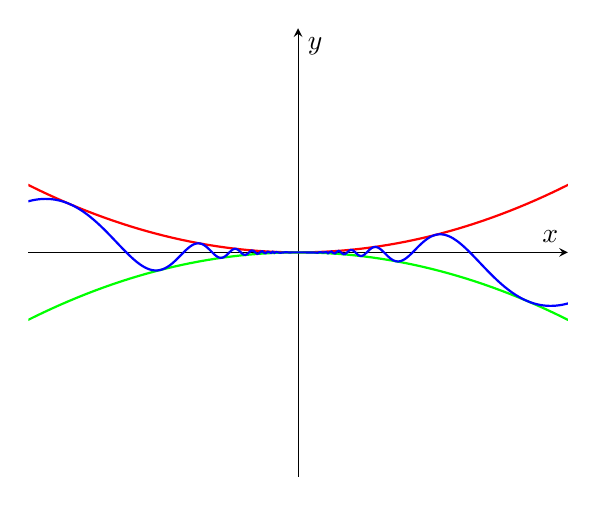
\begin{tikzpicture}
    \begin{axis}[
      ticks=none,
      axis lines=middle,
      axis equal,
      xlabel=\(x\),
      ylabel=\(y\),
      xmin=-0.25,
      xmax=0.25,
      ymin=-0.125,
      ymax=0.125,
      yticklabels={,,},
      xticklabels={,,}
      ]
      % \draw[dashed,thick,color=red] (axis cs: 1, 1.5) -- (axis cs: 1, 0) node[below] (endofplotsquare) {\(x_{1}\)};
      \addplot [
      thick,
      color=red,
      domain=-4:4,
      samples=1000
      ]
      {x^2};
      \addplot [
      thick,
      color=green,
      domain=-4:4,
      samples=1000
      ]
      {-x^2};
      \addplot [
      thick,
      color=blue,
      domain=-4:4,
      samples=5000
      ]
      {x^2 * sin(deg(1/(x)))};
    \end{axis}
  \end{tikzpicture}
\end{center}

\begin{mdframed}
  \underline{The Squeeze Theorem}

  Let \(a, L \in \R\). Let \(f, g, \tand h\) be functions defined near \(a\), except possibly at \(a\).

  If
  \begin{itemize}
    \item \(\DS \exists p > 0 \st 0 < \abs{x - a} < p \implies h(x) \leq g(x) \leq f(x)\)
    \item \(\DS \lim_{x \to a} f(x) = L\)
    \item \(\DS \lim_{x \to a} h(x) = L\)
  \end{itemize}
  Then \(\DS \lim_{x \to a} g(x) = L\)
\end{mdframed}

Since we know that for every \(x \neq 0,~x^{2} \sin \frac{1}{x}\) is ``squeezed'' by \(-x^{2} \tand x^{2}\), we know that \(\DS \lim_{x \to 0} -x^{2} = \lim_{x \to 0} x^{2} = \lim_{x \to 0} \sbr{x^{2} \sin \frac{1}{x}} = 0\).

\subsection{Proof of the Squeeze Theorem}

WTS \(\forall \varepsilon, \exists \delta > 0 \st 0 < \abs{x - a} < \delta \implies \abs{g(x) - L} < \varepsilon\)

\underline{Rough Work}

\(\abs{g(x) - L} < \varepsilon\) is equivalent to \(L - \varepsilon < g(x) < L + \varepsilon\).

We \emph{know} \(0 < \abs{x - a} < p \implies h(x) \leq g(x) \leq f(x)\).

We \emph{know} \(\DS \lim_{x \to a} f(x) = L\). \[\exists \delta_{1} > 0 \st 0 < \abs{x - a} < \delta_{1} \implies L - \varepsilon < f(x) < L + \varepsilon\]

We \emph{know} \(\DS \lim_{x \to a} h(x) = L\). \[\exists \delta_{2} > 0 \st 0 < \abs{x - a} < \delta_{2} \implies L - \varepsilon < h(x) < L + \varepsilon\]

If we combine the inequalities that we know, \(h(x) \leq g(x) \leq f(x)\),  \(f(x) < L + \varepsilon\), \(L - \varepsilon < h(x)\), we can conclude what we need.

Take \(\delta = \min\cbr{\delta_{1}, \delta_{2}, p}\).

\begin{proof} \(\)

  Let \(\varepsilon > 0\).

  Use same \(\varepsilon\) in the definition of \(\DS \lim_{x \to a} f(x) = L\). \(\DS \exists \delta_{1} > 0 \st 0 < \abs{x - a} < \delta_{1} \implies \abs{f(x) - L} < \varepsilon \implies f(x) < L + \varepsilon\)

  Use same \(\varepsilon\) in the definition of \(\DS \lim_{x \to a} h(x) = L\). \(\DS \exists \delta_{2} > 0 \st 0 < \abs{x - a} < \delta_{2} \implies \abs{h(x) - L} < \varepsilon \implies L - \varepsilon < h(x)\)

  Take \(\delta = \min\cbr{\delta_{1}, \delta_{2}, p}\).

  Let \(x \in \R\). Assume \(0 < \abs{x - a} < \delta\). This implies:
  \begin{itemize}
    \item \makebox[4cm][l]{\(0 < \abs{x - a} < \delta_{2}\)} Thus \(L - \varepsilon < h(x)\)
    \item \makebox[4cm][l]{\(0 < \abs{x - a} < p\)} Thus \(h(x) \leq g(x) \leq f(x)\)
    \item \makebox[4cm][l]{\(0 < \abs{x - a} < \delta_{1}\)} Thus \(f(x) < L + \varepsilon\)
  \end{itemize}

  Therefore \(L - \varepsilon < g(x) < L + \varepsilon\). Equivalently, we have proven that \(\abs{g(x) - L} < \varepsilon\), as needed. \qedhere
\end{proof}

\subsection{The definition of continuity}

``A function is continuous when its graph can be drawn without lifting the pen from the paper.''

\begin{mdframed}

  \underline{Definition of Continuity}

  Let \(a \in \R\). Let \(f\) be a function defined, at least, on an interval centered at \(a\).

  We say that \(f\) is continuous when \(\DS \lim_{x \to a} f(x) = f(a)\).
\end{mdframed}

This means:
\begin{enumerate}
  \item The limit exists
  \item \(f(a)\) is defined
  \item \(\DS \lim_{x \to a} f(x) = f(a)\)
\end{enumerate}

\begin{mdframed}

  \underline{An equivalent definition (Epsilon Delta Definition of Continuity)}

  Let \(a \in \R\). Let \(f\) be a function defined, at least, on an interval centered at \(a\).

  We say that \(f\) is continuous at \(a\) when

  \[\forall \varepsilon > 0, \exists \delta \st \abs{x - a} < \delta \implies \abs{f(x) - f(a)} < \varepsilon\]

\end{mdframed}

Continuous at a point: \(f\) continuous at \(c\) means \(\DS \lim_{x \to c} f(x) = f(c)\)

Continuous on an open interval: \(f\) continuous on the interval \((a, b)\) means \(\forall c \in (a, b),~f\) is continuous at \(c\)

Continuous on a closed interval: \(f\) continuous on the interval \([a, b]\) means
\begin{enumerate}
  \item \(\DS \lim_{x \to a^{+}} f(x) = f(a)\)
  \item \(\forall c \in (a, b),~f\) is continuous at \(c\)
  \item \(\DS \lim_{x \to b^{-}} f(x) = f(b)\)
\end{enumerate}

\subsection{The main continuity theorem}

\begin{mdframed}

  \underline{The Main Continuity Theorem}

  Any function we can construct with sum, product, quotient, and composition of polynomials, roots, trigonometric functions, exponentials, logarithms, and absolute values is continuous (on its domain).
\end{mdframed}

Example: \[\lim_{x \to 1} \frac{x^{2} - \sin x}{e^{x} + \ln\br{\sqrt{x} + 3}} = \frac{1 - \sin 1}{e + \ln 4}\]

\subsection{Limits and composition of functions}

We do not have a ``Limit Law'' for compositions. Just knowing that two functions have limits does not guarantee that the composition of the two functions has a limit.

\underline{False Theorem}

If \(\DS \lim_{x \to a} f(x) = L \tand \lim_{y \to L} g(y) = M\)

\(\cancel{\text{Then \(\DS \lim_{x \to a} g(f(x)) = M?\)}}\)

\begin{mdframed}

  \underline{Theorem 1}

  If \(f\) continuous at \(a\), and \(g\) continuous at \(f(a)\)

  Then \(g \circ f\) continuous at \(a\).

\end{mdframed}

% A counter example for the false theorem is as follows.

% \(f(x) = \begin{cases} x \sin \frac{\pi}{x} & \text{ if } x \neq 0 \\ 0 & \text{ if } x = 0 \end{cases}\)

% \(g(y) = \begin{cases} 2 & \text{ if } y = 0 \\ 1 & \text{ if } y \neq 0 \end{cases}\)

% \(g(f(x)) = \begin{cases} 2 & \text{ if } x \dots \\ 1 & \text{ if } x \dots \end{cases}\)

To get to the core of the probelm, we can look at what the theorems are really saying.

\begin{itemize}
  \item \(\DS \lim_{x \to a} f(x) = L\) means:

        \(\cbr{x \text{ close to } a, x \neq a} \implies f(x) \text{ close to } L\).

  \item \(f\) continuous at \(a\) means:

        \(x \text{ close to } a \implies f(x) \text{ close to } f(a)\).
\end{itemize}

Let us look at \emph{Theorem 1}.

The first hypothesis means \(x \text{ close to } a \implies f(x) \text{ close to } f(a)\).

The second hypothesis means \(y \text{ close to } f(a) \implies g(y) \text{ close to } g(f(a))\).

We can concatenate the two implications to form \(x \text{ close to } a \implies g(f(x)) \text{ close to } g(f(a))\).

By contrast, let us try and do the same thing with the \emph{False Theorem}.

The first hypothesis means \(x \text{ close to } a \text{ but } x \neq a \implies f(x) \text{ close to } L\).

The second hypothesis means \(y \text{ close to } L \text{ but } y \neq L \implies g(y) \text{ close to } M\).

We cannot concatenate these two implications as the ``then'' part in the first does not match the ``if'' part in the second. This is why the theorem is false.

But we can fix the theorem!

\begin{mdframed}
  \underline{Theorem 2}

  If
  \begin{itemize}
    \item \(\DS \lim_{x \to a} f(x) = L\)
    \item \(\DS f(x) \neq L\) for \(x\) on an interval centered at \(a\), excepy maybe at \(a\).
    \item \(\DS \lim_{y \to L} g(y) = M\)
  \end{itemize}

  Then \(\DS \lim_{x \to a} g(f(x)) = M\)
\end{mdframed}

\begin{mdframed}
  \underline{Theorem 3}

  If
  \begin{itemize}
    \item \(\DS \lim_{x \to a} f(x) = L\)
    \item \(g\) is continuous at \(L\)
  \end{itemize}

  Then \(\DS \lim_{x \to a} g(f(x)) = g(L)\)
\end{mdframed}

\subsection{Discontinuties (and how to remove them)}
\subsection{A geometric proof for a trigonometric limit}
\subsection{Review of basic techniques for computing limits}
\subsection{How to compute the limit of a rational function at infinity}
\subsection{The Extreme Value Theorem}
\subsection{The Intermediate Value Theorem}

\include{03/03.tex}
\include{04/04.tex}
\include{05/05.tex}
\include{06/06.tex}
\include{07/07.tex}
\include{08/08.tex}
\include{09/09.tex}
\include{10/10.tex}
\include{11/11.tex}
\include{12/12.tex}
\include{13/13.tex}
\include{14/14.tex}

\end{document}
